\subsection{IBM Storage Manager para DS3X00}

Para aceder ao Storage Manager deverá aceder a:

\begin{figure}[H]
    \begin{center}
        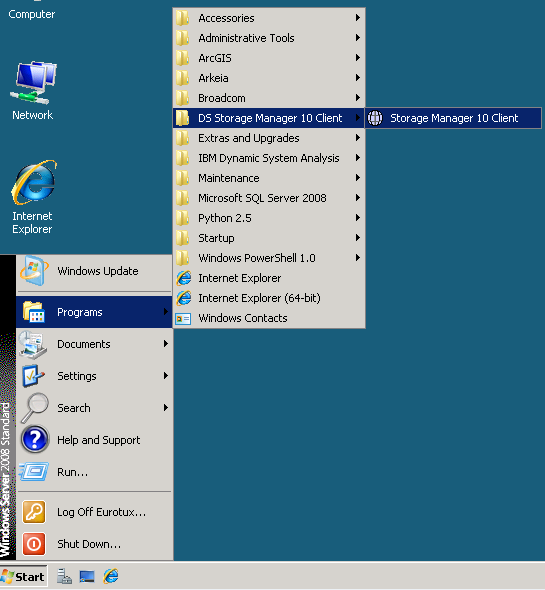
\includegraphics[width=10cm]{include/img/ds3000_win_1}
    \end{center}
    \caption{Menu de acesso a StorageManager}
    \label{fig:ds3000-win-1}
\end{figure}

Deverá ser-lhe apresentada a aplicação Storage Manager, tal como o exemplo seguinte:

\begin{figure}[H]
    \begin{center}
        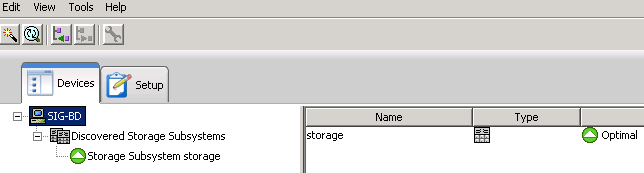
\includegraphics[width=10cm]{include/img/ds3000_win_2}
    \end{center}
    \caption{Ecrã inicial do StorageManager}
    \label{fig:ds3000-win-2}
\end{figure}

Depois deve carregar com o botão direito sobre a storage e escolher "Manage Storage Subsystem"

\begin{figure}[H]
    \begin{center}
        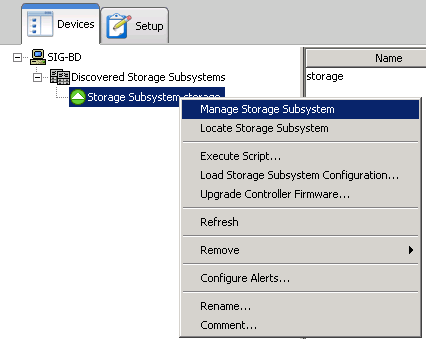
\includegraphics[width=10cm]{include/img/ds3000_win_3}
    \end{center}
    \caption{Acesso a gestão}
    \label{fig:ds3000-win-2}
\end{figure}

De seguida vai-lhe ser apresentado o acesso à gestão da storage.

\begin{figure}[H]
    \begin{center}
        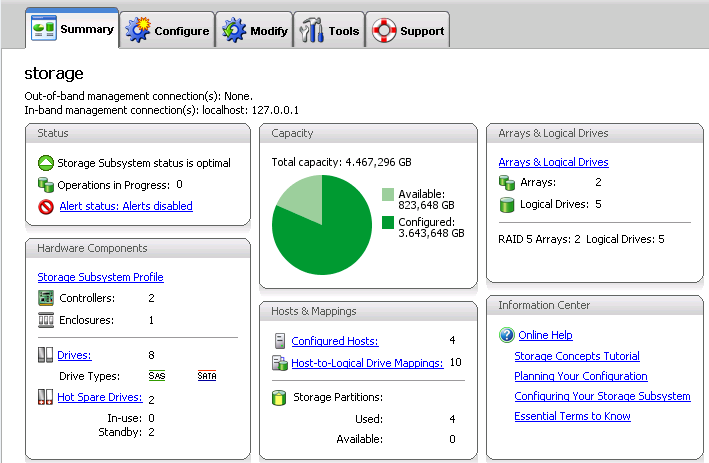
\includegraphics[width=10cm]{include/img/ds3000_win_4}
    \end{center}
    \caption{Ecrã principal de gestão do Storage Manager}
    \label{fig:ds3000-win-4}
\end{figure}

Posteriormente poderá efectuar a gestão da storage. Para mais informações deverá consultar o manual do equipamento.
É importante salientar que a storage pode ser gerida de duas formas:
\begin{itemize}
\item in-band: utiliza a própria ligação em fibra ou SAS para gerir a storage.
\item out-of-band: utiliza a rede para aceder aos controladores da storage para efectuar a sua gestão
\end{itemize}

A grande diferença entre estes dois métodos de gestão prende-se com o facto do primeiro não necessitar de qualquer acesso à rede para efectuar a configuração da storage, utilizando para tal as ligações em FC ou SAS que tem com a storage para a gerir enquanto que o segundo utiliza a rede para gerir a storage. Neste caso a máquina que tem a aplicação de gestão da storage não necessita de qualquer ligação em FC ou SAS à mesma para a gerir.
